% !TEX TS-program = pdflatex
% \documentclass[draftcls, onecolumn, journal]{IEEEtran}
% \documentclass[journal]{IEEEtran}
\documentclass[a4paper,11pt]{article}
%\usepackage{fullpage}

%\renewcommand{\baselinestretch}{1.9}
\usepackage{graphicx}
%\usepackage{cite}
\usepackage[style=ieee, nohashothers=true, nosortothers=true, uniquelist=true, natbib=true, backend=biber, sorting=none]{biblatex}
\DefineBibliographyStrings{english}{andothers={}}

\addbibresource{project.bib}
\DeclareFieldFormat[article]{volume}{Vol. #1}
\DeclareFieldFormat[article]{number}{No. #1}
\DeclareFieldFormat[article]{pages}{p. #1}
\DeclareFieldFormat[inproceedings]{pages}{p. #1}

%\documentclass[journal]{IEEEtran}
\usepackage[a4paper, total={6in, 8.5in}, top=1in, bottom=1in, left=1in, right=1in]{geometry}
\usepackage{mathtools}
\usepackage{amssymb}
\usepackage{amsmath}
\usepackage{pythonhighlight}
\usepackage[utf8]{inputenc}
\usepackage{fancyhdr}
\usepackage{pythonhighlight}
\usepackage{changepage}
\usepackage{slashbox}
\usepackage{floatrow}
\usepackage{listings}
\usepackage[hidelinks]{hyperref}
\usepackage[T1]{fontenc}
\usepackage[utf8]{inputenc}
\usepackage[english]{babel}
\usepackage{csquotes}
\usepackage{booktabs}
\usepackage{multicol}
\usepackage{titlesec}

\setcounter{secnumdepth}{4}
\setcounter{tocdepth}{4}


\titleformat{\paragraph}
{\normalfont\normalsize\bfseries}{\theparagraph}{1em}{}
\titlespacing*{\paragraph}
{0pt}{3.25ex plus 1ex minus .2ex}{1.5ex plus .2ex}

\usepackage{caption}
\usepackage{subcaption}
\usepackage{color} %red, green, blue, yellow, cyan, magenta, black, white
\definecolor{mygreen}{RGB}{28,172,0} % color values Red, Green, Blue
\definecolor{mylilas}{RGB}{170,55,241}


\floatsetup[table]{capposition=top}

\sloppy
\definecolor{lightgray}{gray}{0.5}
\setlength{\parindent}{0pt}
\setlength{\headheight}{14pt}

\renewcommand{\headrulewidth}{.4mm} % header line width
\newcommand{\norm}[1]{\left\lVert#1\right\rVert}

\pagestyle{fancy}
\fancyhf{}
\fancyhfoffset[L]{-1cm} % left extra length
\fancyhfoffset[R]{-1cm} % right extra length
\rhead{\bfseries Kutay U\u{g}urlu 2232841}
\lhead{Deep MLP for Dimensional SER}
\rfoot{}

\DeclarePairedDelimiter\ceil{\lceil}{\rceil}
\DeclarePairedDelimiter\floor{\lfloor}{\rfloor}

\author{Kutay U\u{g}urlu 2232841}

\begin{document}

    
\lstset{language=Matlab,%
    %basicstyle=\color{red},
    breaklines=true,%
    morekeywords={matlab2tikz},
    keywordstyle=\color{blue},%
    morekeywords=[2]{1}, keywordstyle=[2]{\color{black}},
    identifierstyle=\color{black},%
    stringstyle=\color{mylilas},
    commentstyle=\color{mygreen},%
    showstringspaces=false,%without this there will be a symbol in the places where there is a space
    numbers=left,%
    numberstyle={\tiny \color{black}},% size of the numbers
    numbersep=9pt, % this defines how far the numbers are from the text
    emph=[1]{for,end,break},emphstyle=[1]\color{red}, %some words to emphasise
    %emph=[2]{word1,word2}, emphstyle=[2]{style},    
}

\fancyfoot[C]{\thepage}

\title{\LARGE \LARGE EE583 Pattern Recognition Project \\ 
Inspection of \textit{Deep Multilayer Perceptrons for Dimensional Speech Emotion Recognition}}

\maketitle{\LARGE}
\pagebreak
\tableofcontents
\pagebreak

\section{Introduction}

Speech emotion recognition is the task of extracting the emotion category from either text or audio data. It has already some applications in security, medicine, entertainment and education \cite{cen2016real}. 

This project report investigates the idea that Atmaja \textit{et al.}stated in \textit{Deep Multilayer Perceptrons for Dimensional Speech Emotion Recognition}~\cite{atmaja2020deep}. The authors of the study discusses the need of utilizing modern computation units, such as Long Short Term Memory(LSTMs) and Convolutional Neural Networks(CNNs), in the neural networks for the task of dimensional speech emotion recognition. 

The organization of the report is as follows:
\begin{itemize}
    \item The problem and the proposed solutions to it are briefly introduced in this section.
    \item The theory of dimensional and categorical emotions are mentioned in Section \ref{sec:theory}.
    \item The methods, datasets and neural network architectures used in the implementation of the speech emotion recognition can be seen in Section \ref{sec:implementation}.
    \item Section \ref{sec:results} is left for the definition of the evaluation metrics utilized in the study, the reproduced results, evaluation of the models with other datasets and the discussion on the results.  
\end{itemize}

\pagebreak

\section{Theory} \label{sec:theory}

The idea that emotion categories can be separated based on some emotional dimensions dates back to 1979. Russel argued in \cite{russell1979affective} that categorical emotions, namely sadness, anger, joy, etc., can be classified by the values they represent in three dimensions: Valence, Arousal and Dominance.

\begin{figure}[h]
\centering
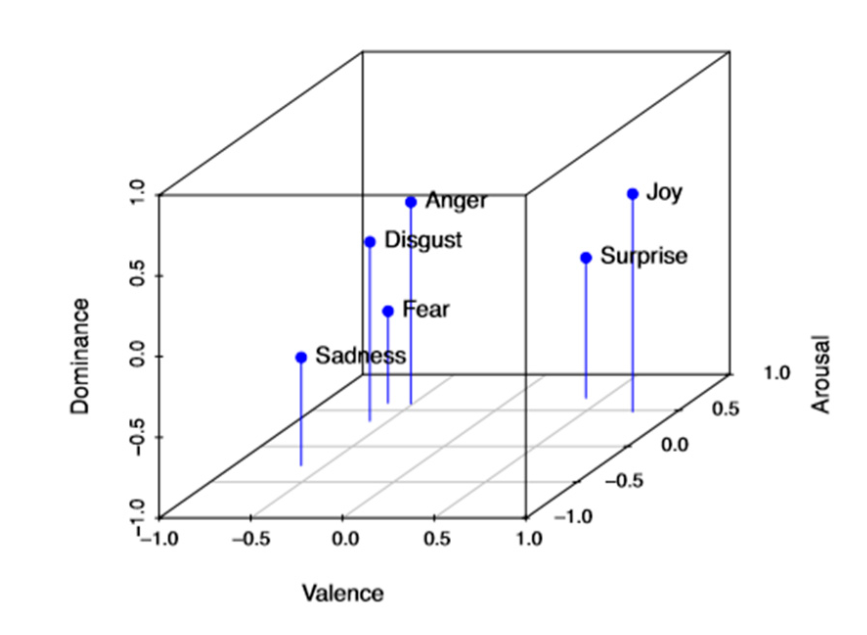
\includegraphics[width=0.8\textwidth]{dimensions_pic.png}
\caption{Categorical Emotions in VAD space \cite{bualan2020emotion}}\label{fig:dimensions}
\end{figure}

\begin{table}[h]
    \centering{
\begin{tabular}{cccc} \toprule \toprule
     & Valence & Arousal & Dominance \\ \midrule
    Anger  & -0.43 & 0.67 & 0.34  \\ \midrule
    Joy  & 0.76  & 0.48 & 0.35   \\ \midrule
    Surprise  & 0.4  & 0.67 & -0.13   \\ \midrule
    Disgust  & -0.6  & 0.35 & 0.11   \\ \midrule
    Fear  & -0.64   & 0.6 & -0.43    \\ \midrule
    Sadness  & -0.63  & 0.27 & -0.33   \\ \bottomrule \bottomrule
\end{tabular}
}
\caption{\label{tab:vadtable}VAD Dimensions of 6 basic emotions \cite{bualan2020emotion}.}
\end{table}


\pagebreak

\section{Implementation} \label{sec:implementation}

This section composes of two sections describing the implementation of the original authors and slight changes made.

\subsection{Original Paper}
\subsubsection{Data} 

\paragraph{Datasets}

There are mainly two datasets utilized in the paper. 
\begin{enumerate}
    \item \textbf{IEMOCAP(The Interactive emotional Dyadic Motion Capture database):} 12 hours of speech data consisting of 10039 utterances  is used \cite{busso2008iemocap}.
    \item \textbf{MSP-IMPROV:} 18 hours of speech data consisting of 8438 utterances is used \cite{busso2016msp}.
\end{enumerate}

\paragraph{Data Preprocessing} \label{subsec:datapreprocess}

The shared data in \cite{atmaja2020deep} are already preprocessed and the scripts and tools the authors utilized was not explicitly shared. However, the types of features Atmaja \textit{et al.} used is shared in the paper.  
The audio in the dataset are used to extract 47 features per utterance.
These features are obtained in a 2-level process. First, the Low Level Descriptors defined in \cite{eyben2010opensmile} are calculated by the \texttt{opensmile} software. These Low Level Descriptors are as follows: 
\begin{multicols}{3}
\begin{itemize}
    \item Intensity
    \item Alpha ratio
    \item Hammarberg index
    \item Spectral slope 0-500 Hz
    \item Spectral slope 500-1500 Hz
    \item Spectral flux
    \item 4 MFCCs
    \item $f_0$
    \item jitter
    \item shimmer
    \item Harmonics-to-Noise Ratio (HNR)
    \item Harmonic difference H1-H2
    \item Harmonic difference H1-A3
    \item F1
    \item F1 bandwidth
    \item F1 amplitude
    \item F2
    \item F2 amplitude
    \item F3 
    \item F3 amplitude
\end{itemize}
\end{multicols}

Then, 47 features, High Statistical Functions of these 23 features are calculated in two sets by utilizing the mean and standard deviation. In addition, authors defined an extra feature: Silence. The silence is defined as the ratio of the silent frames per utterance. 
\begin{equation}
    S = \frac{N_s}{N_t}
\end{equation}
where $N_s$ is the number of silent frames and $N_t$ is the number of total frames.
The framed are labelled as silent by being compared to a threshold. 
\begin{equation}
    Threshold = 0.3 \times X_{RMS}
\end{equation} 
and 
\begin{equation}
    X_{RMS} = \sqrt{\frac{1}{n}\sum_{i=1}^n{x[i]}^2}
\end{equation} 
where the factor 0.3 is determined empirically.
\subsubsection{Models}

The benchmark models which authors use to compare the model performance are composed of CNN and LSTM units. The authors use the same number of units and layers in the model. In Figure \ref{fig:models}, it can be seen that the models have approximately the same number of trainable parameters. 

The multiplayer perceptron models are implemented with scikit-learn's MLP Regressor \cite{scikit-learn} and the remaining CNN and LSTM models are implemented with Tensorflow \cite{tensorflow2015-whitepaper}.

\begin{figure}[h]
\centering
\begin{subfigure}[b]{0.45\textwidth}
\centering
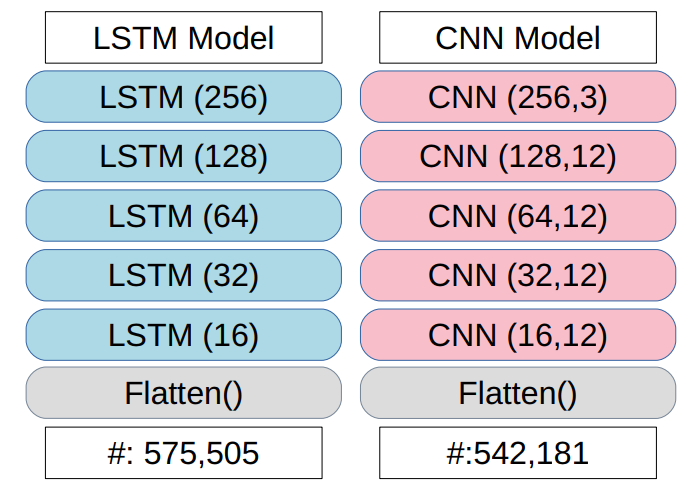
\includegraphics[width=0.8\textwidth, height=5cm]{modelsparams.png}
\caption{Benchmark model architectures}\label{subfig:subcnnlstm}
\end{subfigure}
\begin{subfigure}[b]{0.45\linewidth}
\centering
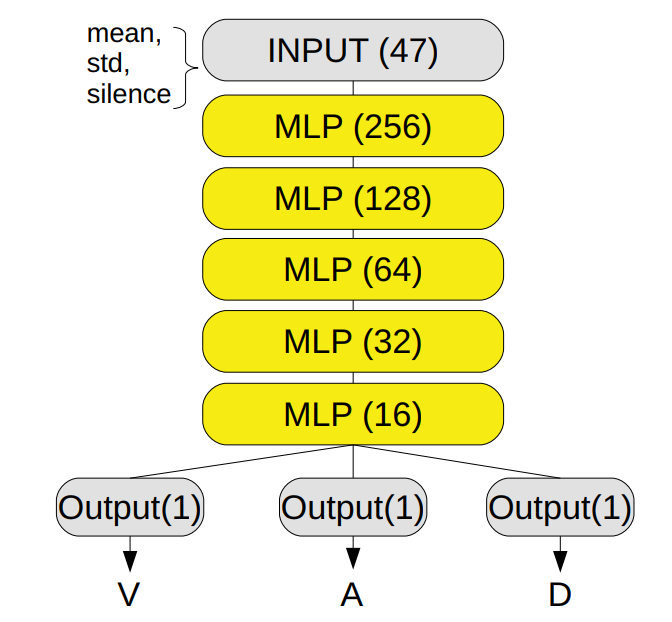
\includegraphics[width=0.8\textwidth]{modelparamsmlp.png}
\caption{Proposed Multilayer MLP architecture}\label{subfig:submlp}
\end{subfigure}
\caption{Model architectures utilized in \cite{atmaja2020deep}}
\label{fig:models}
\end{figure}


\subsection{Changes made}

\subsubsection{Data}

\paragraph{Datasets}

The authors of the study made use of the most of the databases whose utterances are labelled by multiple annotators in the Valence-Arousal-Dominance dimension. 
Although there are many available datasets on Speech Emotion Recognition, only a few of them are labelled in the same manner. However, these datasets were not available for open access. The remaining available datasets are either labelled categorically, \textit{i.e.} sad, joy, anger etc. or labelled only in 2 dimension: Valence and Arousal. Since the latter option requires one to re-train the model and does not provide one with the chance of evaluating the pretrained model with the new test data, categorical dataset, MELD \cite{atmaja2020deep}, was used for the evaluation. The dataset consists of utterances in mp4 format from the TV series ''Friends'' and the categorical emotion regarding these utterances. 

\paragraph{Data Preprocessing}

To augment the dimensional, \textit{i.e.} numerical, labels from the categorical labels. This is conducted by mapping the categorical labels to points in the Valence-Arousal-Dominance space via the mapping given in Table \ref{tab:vadtable} first, and perturbing the points with normally distributed noise with standard deviation 0.01, to reflect the effect of multiple annotators. To get the time series data in WAV format in the same datarate of 44.1 kHz from MP4 format, \texttt{FFMPEG} is utilized.   

The whole data formation process can be seen in Figure \ref{fig:dataformation}.

\begin{figure}[h]
\centering
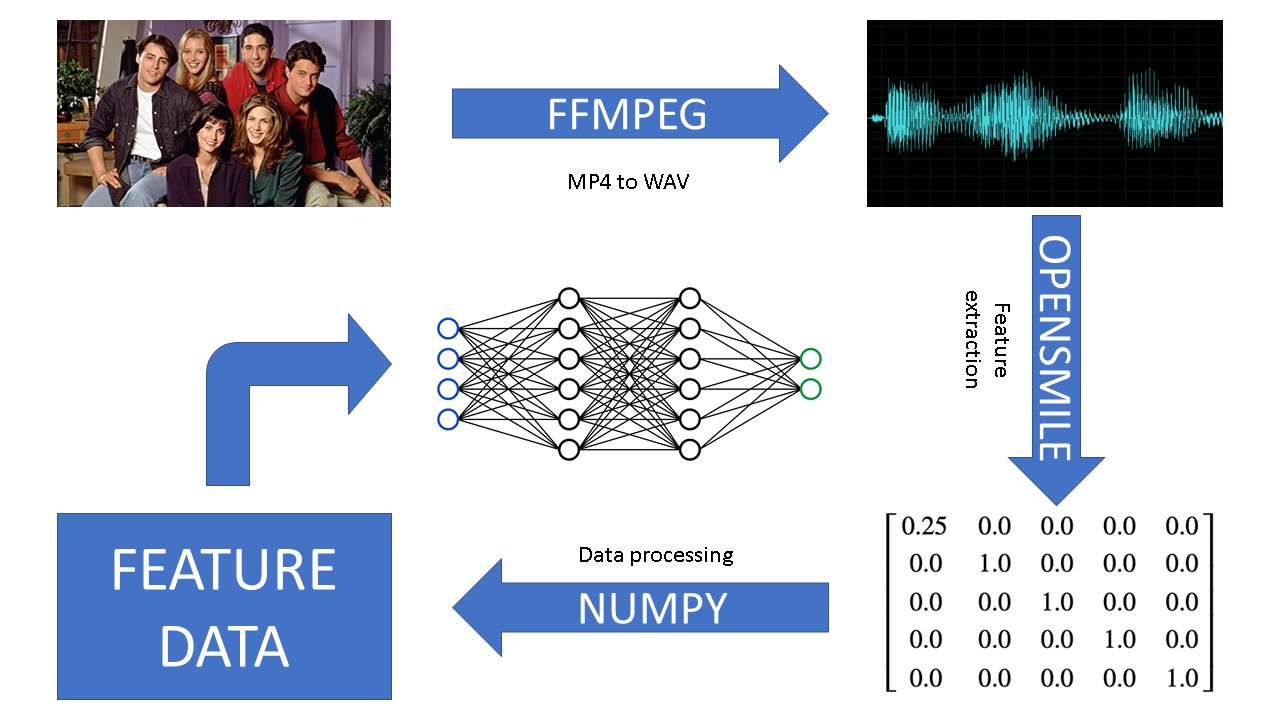
\includegraphics[width=0.8\textwidth]{Presentation.png}
\caption{The data formation steps used to augment data from MELD dataset}\label{fig:dataformation}
\end{figure}

\pagebreak

\subsubsection{Models}

The pre-trained models are evaluated using the new test data. Furthermore, to make better conclusions on the models' capability to fit the data, the data is split to train, test and validation sets and the model is evaluated after being retrained. The architectures of the model were not changed. The only change made was the number of training and patience epoch for early stopping. 


\section{Results and Discussion} \label{sec:results}

\pagebreak

\printbibliography

\end{document}